\chapter{Axions in Cosmology}

\begin{figure}[t!]
\begin{aside}[Terminology from cosmology]
\begin{itemize}[leftmargin=0.75em]\setlength\itemsep{0.25ex}
	\item \emph{thermalisation}
---	the process of a particle species reaching thermal equilibrium (i.e., uniform energy and abundance) over cosmological scales, mitigated by self-interactions or processes involving other matter species which diffuse energy.
	\item \emph{freeze-out}
---	the point beyond which the rates of thermalising processes become negligible due to a sufficiently large rate of cosmic expansion, resulting in persistent non-equilibrium distributions of a particle species.
Since the universe cools as it expands, freeze-out may be viewed as the change of phase of a species from a gas to a cooler condensate.
\end{itemize}
\end{aside}
\end{figure}

With the advent of precision cosmology, particle physicists can use the entire universe as a laboratory for ever more sensitive experiments.

[Role of axions: possible dark matter candidates]

Many cosmological tests of axion-like particles involve predicting relative particle abundances in the universe at various epochs, such as the baryon-to-photon or neutrino-to-photon ratios.
Such arguments begin with a minimal `thermodynamical' model of the universe as a homogeneous, isotropic, expanding background upon which different particle species exist uniformly distributed and in thermal equilibrium.
The universe's macrostate is characterised by each species' abundance and energy distribution.
Interactions and processes between species, which at any time may depend on present particle abundances and energies, define differential relations which can be solved to determine the abundance of each species at any point in the universe's evolution.

The assumptions of isotropy and homogeneity specify a spacetime with a Friedmann--Lemaître--Robertson--Walker (FLRW) metric,
\begin{align}
	% \ts g = -c^2 \ts\dd t\otimes\ts\dd t + a(t)^2\qty(η_{ij}\,\ts\dd x^i\otimes\ts\dd x^j)
	\ts g = -c^2 \ts\dd t^2 + a(t)^2\qty(\frac{\ts\dd r^2}{1 - kr^2} + r^2 \ts Θ)
\end{align}
where $k \in \qty{+1, 0, -1}$ reflects the type of spatial curvature, $\ts Θ = \ts\dd θ^2 + \sinθ\,\ts\dd φ^2$ is the metric of the unit sphere, and $\ts\dd x^2 \equiv \ts\dd x\otimes\ts\dd x$.
Standard cosmological models have flat spatial curvature, $k = 0$.
The scale factor $a(t)$ describes the cosmological evolution of the universe and defines the \emph{Hubble parameter,} $H \coloneqq \dot{a}/a$, or cosmic expansion rate.
If the rate $Γ$ of a particle interaction is large (corresponding to large probability per unit spacetime volume for the interaction to occur), then it will provide a mechanism for thermalisation of the species involved---or in the case of production and decay processes, will drive the species to abundance or extinction. 
If the rate is smaller than the rate of cosmic expansion, $Γ \ll H$, then the interaction or process will freeze-out and become negligible.
If a species' most dominant interactions freeze-out, then it becomes thermally isolated from other fields and its abundance remains fixed.


\section{Axion Interactions and Processes}

\begin{figure}[h]
	\centering
	\begin{subfigure}[]{0.3\textwidth}
		\centering
		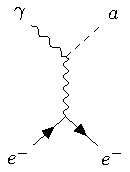
\includegraphics{diagrams/primakoff-process.pdf}
		\caption{Primakoff}
		\label{fig:Primakoff}
	\end{subfigure}
	\begin{subfigure}[]{0.3\textwidth}
		\centering
		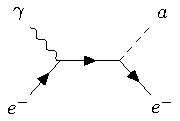
\includegraphics{diagrams/compton-process.pdf}
		\caption{Compton}
		\label{fig:Compton}
	\end{subfigure}
	\caption{Dominant axion processes with electrons (or positrons with arrows reversed).}
	\label{fig:axion-biphoton}
\end{figure}


\begin{align}
	Γ_{a\to γγ} \approx \SI{1.1e-24}{\per\second}\qty(\frac{m_a}{\si{\eV}})^5
\end{align}

